\chapter{MARCO TEÓRICO} 
	
	\vspace{0pt}
	
	\section{LOGÍSTICA DEL TRANSPORTE DE PASAJEROS}
	\subsection{Logística}
		``Logística es planificar, operar, controlar y detectar oportunidades de mejora del proceso de flujo de materiales (insumos, productos), servicios, información y dinero.  Es la función que normalmente opera como nexo entre las fuentes de aprovisionamiento y suministro y el cliente final o la distribución.  Su objetivo es satisfacer permanentemente la demanda en cuanto a cantidad, oportunidad y calidad al menor costo posible para la empresa.''\parencite{carro2013logistica}
	\subsection{Transporte}
		Según \textcite{koch2001transporte}: ``El concepto de “transporte” hace referencia al traslado de personas y mercancías de un lugar a otro por diversas razones en el menor tiempo posible. En el caso de las personas, destacan los motivos laborales, de estudio o de satisfacción de otras necesidades como el ocio, el acceso a servicios de salud, entre otros; en
		el caso de las mercancías, la necesidad de producción de bienes industriales y de consumo y la posterior comercialización de estos hacen del proceso de transporte un elemento central.'' Por su parte en la \textcite{ley2011transporte}: ``Se denomina transporte al traslado de un lugar a otro de personas y carga.''
		
		
		El transporte es un componente de la logística, que se refiere al conjunto de recursos y estrategias utilizados para organizar un servicio o administrar una empresa. En el ámbito comercial, la logística se relaciona con el envío de productos al lugar adecuado, en el momento correcto y bajo las condiciones necesarias. Por lo tanto, el transporte de mercancías es una parte integral de la logística. El propósito de una empresa es asegurar que la distribución y venta de sus productos se realice de manera eficiente y al menor costo posible. En este contexto, el transporte abarca tanto los vehículos como las infraestructuras asociadas, como camiones, barcos, trenes de carga, carreteras y puertos.
		
		También existen dos tipos de transporte, el público y el privado.
		
		Se habla de transporte público, para hacer referencia a los autobuses, trenes y otras unidades móviles que sirven para la movilización de los ciudadanos de una comunidad y que está solventado y manejado por el Estado vigente. Cabe señalar que en algunos casos, dichos coches pertenecen a empresas privadas que tienen algún tipo de acuerdo con el gobierno y han asumido la responsabilidad de brindar un servicio determinado a la comunidad. Resulta importante señalar que esta clase de transporte no tiene como propósito la generación de ganancias, sino que debe cumplir con un fin social y ser útil para la comunidad. Por ejemplo: “Los transportes públicos están colapsados y requieren de mayores inversiones para
		poder satisfacer las necesidades de la población”.
		
		El transporte privado, en cambio, es el que pertenece a individuos o empresas particulares. En este caso los responsables de la manutención de dichos vehículos son sus dueños, al igual que serán quienes respondan por ellos en caso de
		accidente.
	\subsection{Pasajero}
		En la \textcite{ley_municipal2012transporte} en su artículo 59 se define a los usuarios o pasajeros como ``Las personas naturales o jurídicas que utilizan un vehículo del servicio público o privado de transporte, para trasladarse de un origen a un destino a cambio de una tarifa establecida o remuneración convenida, son considerados usuarios o pasajeros en el marco de la presente Ley Municipal.''
	
	\subsection{Sistema de transporte}
		De acuerdo con \textcite{garcía2016gestión}: ``Un sistema de transporte desde la perspectiva informática es una red interconectada de componentes físicos y digitales que utiliza tecnologías avanzadas de información y comunicación para optimizar el flujo de personas y mercancías. Incluye sistemas de gestión de tráfico, planificación de rutas en tiempo real, control de flotas y plataformas de información al usuario, todos ellos integrados mediante software especializado y bases de datos.''
	% \subsection{Funcionalidad del transporte}
	\section{RESERVA Y VENTA DE PASAJES}
	\subsection{Proceso de reserva y venta de pasajes}
		El proceso de reserva y venta de pasajes es un componente fundamental en la operación de cualquier empresa de transporte de pasajeros. Según \textcite{aparicio2013gestion}, este proceso implica una serie de pasos secuenciales que permiten al cliente asegurar su lugar en un viaje específico. Tradicionalmente, las empresas de transporte han utilizado diversos canales para la reserva y venta, incluyendo puntos de venta físicos, call centers, y más recientemente, plataformas en línea.	
	\subsection{Emisión y gestion de boletos}
		La emisión y gestión de boletos es un proceso crítico que ha evolucionado significativamente con la tecnología. \textcite{agenjo2008transporte} describen dos tipos principales de boletos en el transporte moderno: los electrónicos (e-tickets) y los impresos tradicionales. Independientemente del formato, los boletos deben contener información esencial como datos del pasajero, detalles del viaje, asiento asignado y un método de validación.
		
		El proceso de emisión, según \textcite{garcía2016gestión}, debe ser ágil y estar vinculado directamente con la confirmación del pago. La gestión eficiente de boletos implica un sistema robusto de validación, ya sea en terminales o a bordo de los vehículos, así como la capacidad de reimpresión en caso de pérdida. Además, como señala \textcite{robuste2005logistica}, el seguimiento y registro de los boletos emitidos es importante para el control operativo y financiero de la empresa de transporte.
	\subsection{Cambios y cancelaciones}
		La gestión de cambios y cancelaciones es un aspecto delicado que requiere un equilibrio entre la flexibilidad para los clientes y la protección de los intereses de la empresa. Según \textcite{tejero2015transporte}, las políticas de cambios y cancelaciones deben ser claras, especificando plazos permitidos y cargos aplicables.
		
		El proceso de solicitud de cambios, como describe \textcite{ramírez2015logística}, implica la verificación de disponibilidad para nuevas fechas y el cálculo de diferencias tarifarias. En cuanto a las cancelaciones, el sistema debe determinar el monto del reembolso según la política establecida. La gestión de reembolsos, de acuerdo con \textcite{garcía2016gestión}, debe ser eficiente y transparente, ofreciendo múltiples métodos según las preferencias del cliente.
		
		Un aspecto importante señalado por \textcite{rivera2002ESTUDIODL} es la reasignación de asientos liberados, lo que permite optimizar la ocupación de los vehículos. Además, el registro detallado de cambios y cancelaciones proporciona datos valiosos para el análisis de patrones de comportamiento de los clientes y la mejora continua de los servicios.
		
		En conjunto, estos procesos de reserva, emisión de boletos y gestión de cambios y cancelaciones forman la columna vertebral de la operación de venta de pasajes en una empresa de transporte. Su eficiente implementación y gestión son cruciales para la satisfacción del cliente y el éxito operativo de la empresa.
	\section{LOGÍSTICA DE ENVÍO DE ENCOMIENDAS}
	\subsection{Encomienda}
		La encomienda es el objeto o paquete que se transporta de un punto a otro a través de un servicio de mensajería o transporte. Según \textcite{stock2000strategic}, ``una encomienda representa una unidad logística que debe ser gestionada y tratada como tal, garantizando su integridad desde el origen hasta el destino final''. En el contexto del transporte de encomiendas, es fundamental contar con un sistema que permita la correcta identificación, seguimiento y gestión de cada paquete.
		
		\textcite{garcía2016gestión} destaca que el concepto de encomienda ha evolucionado con el tiempo, especialmente con el auge del comercio electrónico. Actualmente, las empresas de transporte deben estar preparadas para manejar una amplia gama de artículos, desde documentos hasta productos perecederos, cada uno con sus propios requisitos de manipulación y transporte. Esta diversidad exige sistemas flexibles y adaptables que puedan responder a las necesidades cambiantes de los clientes y del mercado.
	\subsection{Proceso de recepción}
		El proceso de recepción es la primera etapa en la gestión de encomiendas, donde se verifica la información proporcionada por el remitente, se inspecciona el paquete y se registran los detalles necesarios para su envío. De acuerdo con \textcite{garcía2016gestión}, este proceso implica la verificación inicial del paquete, el registro de información relevante y la asignación de un identificador único. \textcite{escudero2019logistica} enfatiza la importancia de este paso para garantizar la trazabilidad y el manejo adecuado de la encomienda durante todo su trayecto.
		
		Con el avance de las tecnologías, muchas empresas han implementado sistemas que automatizan el proceso de recepción, permitiendo la digitalización de la información desde el inicio del proceso logístico. Esto facilita un flujo continuo de datos entre las distintas etapas del envío, reduciendo errores humanos y optimizando los tiempos de procesamiento.
	\subsection{Clasificación de encomiendas}
		La clasificación de encomiendas es un paso fundamental para optimizar el proceso de envío. Según \textcite{i2001manual}, las encomiendas se pueden clasificar según diversos criterios, como tamaño, peso, destino, urgencia o tipo de contenido. \textcite{tejero2015transporte} señala que una clasificación eficiente permite una mejor planificación de rutas y utilización de los espacios de carga.
		
		\textcite{escudero2019logistica} agrega que la clasificación también juega un papel crucial en la priorización de los envíos y la asignación de recursos. Por ejemplo, las encomiendas urgentes o perecederas pueden requerir un tratamiento especial y rutas más directas. Además, una clasificación adecuada facilita el cumplimiento de regulaciones específicas, como las relacionadas con el transporte de mercancías peligrosas o artículos restringidos.
	\subsection{Embalaje y etiquetado}
		El embalaje y etiquetado son procesos críticos para garantizar la integridad y correcta identificación de las encomiendas. \textcite{ramírez2015logística} destaca que el embalaje debe proporcionar protección adecuada según la naturaleza del contenido y las condiciones del transporte. Esto puede incluir el uso de materiales de amortiguación, envoltorios impermeables o contenedores especializados para artículos frágiles o sensibles a la temperatura.
		
		El etiquetado, por su parte, es igualmente importante, ya que proporciona la información necesaria para la correcta identificación del paquete. Esta información incluye los datos del remitente y del destinatario, instrucciones especiales de manejo y, en muchos casos, códigos de seguimiento que permiten rastrear el paquete en tiempo real. \textcite{ballou2004logistica} menciona que un etiquetado claro y preciso es esencial para evitar errores en la clasificación y garantizar que el paquete llegue a su destino de manera eficiente. Las tecnologías modernas, como los códigos QR, también han facilitado este proceso, permitiendo una gestión más ágil de los envíos.
	\subsection{Entrega al destinatario}
		La entrega al destinatario es la fase final en la logística de encomiendas, y su éxito depende en gran medida de la eficiencia de los pasos previos. Según \textcite{garcía2016gestión}, este proceso implica la verificación de la identidad del destinatario, la obtención de una firma de recepción y la resolución de cualquier incidencia que pueda surgir. \textcite{tejero2015transporte} resalta la importancia de la puntualidad y la integridad de la entrega como factores clave en la satisfacción del cliente y la reputación de la empresa de transporte.
		
		Sin embargo, la entrega puede enfrentarse a diversos retos, como la ausencia del destinatario en el momento de la entrega o dificultades de acceso en ciertas áreas geográficas. Para contrarrestar estos problemas, empresas líderes en logística han implementado políticas de entrega flexible, que permiten a los clientes seleccionar franjas horarias de entrega, puntos de recogida o reprogramar la entrega.
	\section{GESTIÓN DE BUSES}
	\subsection{Asignación de rutas}
		La asignación de rutas es uno de los procesos clave en la gestión de transporte de pasajeros, ya que su correcta planificación puede mejorar significativamente la eficiencia operativa y la satisfacción del cliente. Según \textcite{molinero2005transporte}, este proceso implica la determinación de los recorridos óptimos que deben seguir los vehículos para cubrir la demanda de pasajeros de manera eficiente. Los autores señalan que una asignación de rutas efectiva debe considerar factores como la densidad poblacional, los patrones de viaje de los usuarios, la infraestructura vial disponible y las restricciones operativas de la empresa.
		
		También \textcite{ballou2004logistica} destaca que la planificación de rutas tiene como objetivo maximizar la eficiencia operativa mediante la reducción de distancias y tiempos muertos. Ballou resalta que una asignación óptima de rutas no solo mejora la utilización de los vehículos, sino que también contribuye a una mejor satisfacción del cliente, al reducir los tiempos de entrega y los costos asociados.
	\subsection{Programación y asignación de conductores}
		La programación y asignación de conductores es un componente esencial en la gestión de buses, que busca optimizar el uso del recurso humano y garantizar la operación eficiente de los servicios. Según \textcite{mauttone2002diseno}, este proceso implica la optimización de recursos humanos para garantizar la cobertura eficiente de las rutas y horarios establecidos. \textcite{ibarra2012synchronization} enfatizan la importancia de sincronizar los horarios de los conductores con los tiempos de llegada y salida de los vehículos, lo que no solo mejora la puntualidad del servicio, sino que también reduce los tiempos de espera para los pasajeros. Esta sincronización debe tener en cuenta factores como los períodos de descanso obligatorios, los cambios de turno y las variaciones en la demanda de pasajeros a lo largo del día.
		
		Por otro lado, \textcite{molinero2005transporte} añaden que la programación debe considerar no solo la eficiencia operativa, sino también el bienestar de los conductores, incluyendo aspectos como la fatiga, las preferencias personales y el equilibrio entre trabajo y vida personal. Esto subraya la necesidad de un enfoque holístico que balancee las necesidades operativas con las consideraciones humanas en la gestión del personal de transporte público.	
	
	\section{MARCO LEGAL Y NORMATIVO}
	\subsection{Autoridad de regulación y fiscalización de telecomunicaciones y transportes}
	La Autoridad de Regulación y Fiscalización de Telecomunicaciones y Transportes
	(ATT), es una institución pública, técnica y operativa, con personalidad jurídica y patrimonio propio, independencia administrativa, financiera, legal y técnica, transitoriamente dependiente del Ministerio de Obras Públicas, Servicios y Vivienda, de acuerdo a la Ley 164.
	
	La ATT, tiene como objetivo regular las actividades que realizan las personas
	naturales y jurídicas, privadas, comunitarias, públicas, mixtas y cooperativas en los sectores de telecomunicaciones, transportes, tics y servicios postales, asegurando que se garantice los intereses y derechos de los consumidores y usuarios, los intereses del país y el desarrollo del sector, promoviendo la economía plural e inclusiva prevista en CPE, y brindando posibilidades para que más habitantes puedan acceder a los servicios \parencite{institucion2017memoria}.
	\subsection{Ley general del transporte}
	"Ley Nro. 165 de transporte, El Sistema de Transporte Integral - STI, en todo el 	Estado Plurinacional de Bolivia, se rige por la Constitución Política del Estado, los Tratados, Convenios e Instrumentos Internacionales, la Ley Marco de Autonomías y Descentralización, la presente Ley, normas sectoriales y otras normas específicas del ordenamiento jurídico del Estado Plurinacional.” \parencite{ley2011transporte}
	
	Sus principios son:
	
	\textbf{Accesibilidad.} Todas las usuarias y usuarios podrán acceder al Sistema de
	Transporte Integral - STI, por el medio y modalidad que escojan, los mismos que
	deben contar con facilidades de acceso y estar en condiciones de equidad, calidad y seguridad.
	
	\textbf{Calidad.} El Sistema de Transporte Integral - STI, debe proveer un servicio en
	conformidad a los requisitos y estándares que garanticen un nivel de servicio
	adecuado de bienestar, eficiencia y eficacia, de acuerdo a la contraprestación
	autorizada.
	
	\textbf{Continuidad.} El Sistema de Transporte Integral - STI, debe funcionar de manera
	permanente, regular y continua.
	
	\textbf{Eficacia.} El servicio de transporte debe cumplir el propósito para el cual fue convenido.
	
	\textbf{Eficiencia.} El Sistema de Transporte Integral - STI, debe prestar servicios en condiciones que garanticen el menor costo operacional y tiempo posible, contemplando un nivel de equidad, calidad y seguridad.
	
	\textbf{Participación y control social.} Se garantizará y facilitará la participación y control social sobre la gestión pública por parte de la sociedad civil organizada.
	
	\textbf{Seguridad.} El Sistema de Transporte Integral - STI, debe prestar servicios en condiciones que garanticen la integridad de personas y carga durante el traslado del lugar de origen al lugar de destino.
	
	\textbf{Sostenibilidad.} El sistema de transporte debe prestar servicios que garanticen el menor impacto sobre la salud y el medio ambiente local y global. En el corto, mediano y largo plazo, sin comprometer el desarrollo de futuras generaciones.
	
	\textbf{Transparencia.} Se garantiza la transparencia en el Sistema de Transporte Integral - STI.
	
	\textbf{Universalidad.} Todas las usuarias y usuarios sin distinción alguna, tienen el derecho de utilizar el Sistema de Transporte Integral - STI, para su libre movilidad.
	
	\subsection{Reglamento regulatorio de transporte terrestre de pasajeros y carga}
	
	Resolución Ministerial N° 266 del 14 de agosto de 2017, emitida por el Ministerio de Obras Públicas, Servicios y Vivienda.
	
	\textbf{ARTÍCULO 1 (OBJETO.-)} Reglamentar los aspectos regulatorios del servicio de
	transporte en la modalidad terrestre de pasajeros y carga en aplicación a la Ley N° 165 General de Transporte.
	
	SECCIÓN III: DE LA INFORMACIÓN AL USUARIO Y LAS CONDICIONES	PARA EL VIAJE
	\textbf{ARTÍCULO 14. (INFORMACIÓN AL USUARIO).}
	
	\begin{enumerate}[label=\Roman*., nosep] % Enumeración principal en números romanos
		\item El operador, previamente a la compra del pasaje, debe informar al usuario, de forma clara, precisa y oportuna, sobre lo siguiente:
		\begin{enumerate}[label=\alph*), nosep] % Subítems con letras minúsculas
			\item Destinos, itinerario, rutas, tiempo de viaje, hora de salida y hora estimada de arribo del vehículo al lugar de destino.
			\item Capacidad del vehículo y asientos disponibles de acuerdo a numeración.
			\item Tarifas aprobadas por la Autoridad Regulatoria de acuerdo a las características del servicio de transporte terrestre interdepartamental.
			\item Peso, volumen y cantidad permitidos para el transporte de equipaje facturado y de mano, restricciones del equipaje considerado peligroso y/o nocivo a la salud.
			\item Condiciones del transporte requisitos y documentación necesaria para el viaje al país de destino; condiciones de reembolso en caso que el usuario desista del viaje; entre otros.
		\end{enumerate}
		
		\item El operador tiene la obligación de informar al pasajero antes del inicio y durante el viaje lo siguiente:
		\begin{enumerate}[label=\alph*), nosep]
			\item Características del servicio: destino, fecha, hora del viaje, número y categoría del bus y número de carril.
			\item Derechos y obligaciones de los usuarios.
			\item  Demoras y/o cancelaciones, nueva hora de salida u otros aspectos relacionados al viaje.
			\item Rutas alternativas o desvíos y demoras del viaje por caso fortuito o fuerza mayor durante el viaje.
		\end{enumerate}
	\end{enumerate}
	
	\textbf{ARTÍCULO 15. (ACREDITACIÓN DE INFORMACIÓN PROPORCIONADA AL USUARIO).}
	
	El operador deberá aplicar diferentes mecanismos para brindar información confiable al usuario al momento de la compra del boleto, antes y durante la ejecución del servicio, y al momento de la entrega de carga y/o encomiendas, debiendo cumplir con esta obligación y acreditar tal situación.
	
	\textbf{ARTÍCULO 16. (MECANISMOS DE INFORMACIÓN).}
	
	En los monitores internos del vehículo del operador deben difundir material audiovisual, que informe y dé a conocer a los usuarios sus derechos, obligaciones y prohibiciones.
	
	\textbf{SECCIÓN IV: DEMORA, INTERRUPCIÓN Y/O CANCELACIÓN DEL VIAJE}
	
	\textbf{ARTÍCULO 23. (ATENCIONES AL PASAJERO POR CAUSAS ATRIBUIBLES AL OPERADOR).}
	
	\begin{enumerate}[label=\Roman*.,
		nosep, % Elimina espacio arriba y abajo de la lista
		itemsep=0pt, % Elimina espacio entre los ítems
		parsep=0pt % Elimina espacio entre párrafos dentro de los ítems
		]
		\item En casos de cancelaciones, interrupciones, demoras, duplicidad de boletos o ante cualquier otro evento que sea imputable al operador, éste deberá:
		\begin{enumerate}[label=\alph*),
			nosep, % Elimina espacio entre subítems y la lista
			itemsep=0pt, % Elimina espacio entre los subítems
			parsep=0pt % Elimina espacio entre párrafos dentro de los subítems
			]
			\item Demoras: si la demora fuera mayor a los 15 minutos, informar a los pasajeros la causa y la nueva hora de salida del bus.
			
			Si la demora fuera mayor a una (1) hora, deberán poner a disposición de los pasajeros otro bus de la misma categoría o acordar el transporte de éstos con otro operador.
			
			\item Cancelación: si el viaje es cancelado, deberá embarcar al pasajero en el siguiente bus disponible o de otro operador de idéntica categoría lo más rápidamente posible o en una fecha posterior que convenga al pasajero.
			
			\item Interrupción del viaje: si el viaje es interrumpido después de iniciado por fallas mecánicas y/o accidentes y no pueda continuar el recorrido, el operador se comunicará con su Centro de Contingencias e informará a los pasajeros las medidas a adoptar para auxiliarlos y el tiempo estimado en que llegará el auxilio para continuar el viaje, a fin de que el pasajero tome una determinación: esperar el bus de auxilio o tomar otro medio de transporte para llegar a destino.
			
			\item Duplicación de asientos: ante la venta de dos o más boletos para un solo espacio, deberá asignar al pasajero otro espacio en el bus o embarcarlo en otro bus de igual categoría. Solo a solicitud del usuario deberá rembolsar el 100 por ciento del valor del pasaje.
			
			\item Anticipación del viaje: en caso que el operador anticipe el viaje sin avisar al pasajero, deberá proporcionarle un espacio en el siguiente viaje que le resulte conveniente a su destino final. En estos casos, el pasajero no pagará ningún excedente si el nuevo espacio correspondiera a una tarifa superior. 
		\end{enumerate}
		
		\item En todos los casos, el operador está terminantemente prohibido de recurrir directamente a la devolución; deberá agotar todas las posibilidades para cumplir con el contrato; optará por la devolución únicamente si el pasajero lo requiere.
		
		\textbf{ARTÍCULO 56.- (PROHIBICIONES DEL CONDUCTOR)}
		
		Queda terminantemente prohibido a los conductores de las unidades de servicio de transporte automotor público terrestre en corresponsabilidad con el operador, lo siguiente:
		
		\begin{enumerate}[label=\alph*),
			nosep,
			itemsep=0pt,
			parsep=0pt
			]
			\item Presentarse al trabajo con síntomas de haber ingerido bebidas alcohólicas, o bajo la influencia de sustancias psicotrópicas o ingerirlas en horas de trabajo.			
			\item Transportar pasajeros en los pasillos, buzones y cabina del bus.
			\item Realizar paradas no programadas o desviar el vehículo de su recorrido oficial, a menos que fuera instrucción de las autoridades correspondientes.
			\item Abandonar el vehículo en plena carretera.			
			\item Efectuar paradas no autorizadas cuya duración exceda los 20 minutos.
			\item Agredir físicamente o psicológicamente a los usuarios, personal de la Autoridad Competente, Policía Boliviana u operador del servicio de Terminal Terrestre.			
			\item Usar radios o parlantes con alto volumen de sonido.
			
		\end{enumerate}
		
	\end{enumerate}
		
	\section{INGENIERÍA DE SOFTWARE}
		La Ingeniería de Software es una disciplina dentro de la informática encargada de la aplicación de un enfoque sistemático y metodológico al desarrollo, operación y mantenimiento de sistemas de software de alta calidad. Este campo surgió en respuesta a la creciente complejidad de los sistemas informáticos y a la necesidad de garantizar que los programas y aplicaciones sean confiables, eficientes y ajustados a los requisitos del cliente.
		
		Según \textcite{sommerville2011introduccion}, la ingeniería de software implica la aplicación de principios científicos y de ingeniería en el diseño, desarrollo, prueba y mantenimiento de software. Este enfoque abarca desde el análisis de requisitos, la creación de modelos, la implementación del software, hasta la prueba y verificación del mismo. La clave de la ingeniería de software radica en estructurar cada etapa del proceso de desarrollo de manera que permita crear sistemas que sean fácilmente mantenibles y adaptables a los cambios.
		
		Además, \textcite{pressman2010ingenieria} enfatiza que la ingeniería de software no solo se ocupa del código, sino que integra el manejo de proyectos, la gestión de riesgos y la implementación de técnicas para la verificación de la calidad del producto. Esta disciplina ayuda a gestionar el ciclo de vida completo del software, desde el diseño hasta el mantenimiento, lo cual es esencial en proyectos complejos que requieren altos estándares de calidad y funcionalidad.
		
	\section{MODELO EN CASCADA}
	\subsection{Requerimientos del software}
	\subsection{Diseño del programa}
	\subsection{Codificación}
	\subsection{Construcción y pruebas}
	\subsection{Implantación}
	\section{MODELO ENTIDAD - RELACIÓN}
	\section{BASE DE DATOS}
	\section{HERRAMIENTAS DE DESARROLLO}
	\section{PRUEBAS}
	\section{MODELO DE CALIDAD BOEHM}
		
	
	

	
	
	%\vspace{0.3cm} % Agregar 1 cm de espacio entre el párrafo y la figura
	
	%	\begin{figure}[h] % 'H' del paquete 'float' para mantener posición	
		%		\caption[Descripción corta]
		%		{\newline Resultados del informe PISA 2022.} % Leyenda en la parte superior
		%		\centering
		%		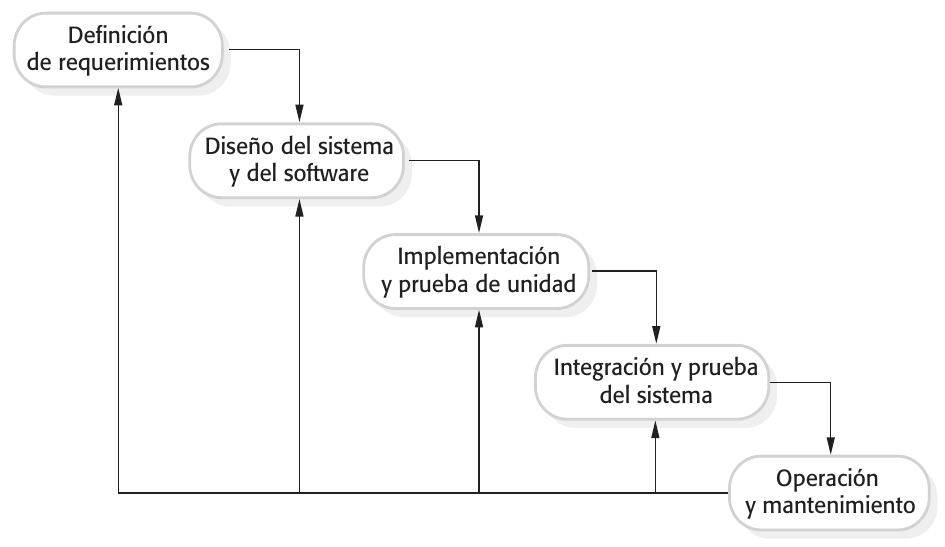
\includegraphics[width=0.95\textwidth]{imagenes/figura2_1.png} % Inserta una imagen
		%		
		%		\begin{flushleft}
			%			\hspace{1.20cm} \textit{Nota.} al pie asociada con esta figura, explicando detalles adicionales. % Nota al pie para esta figura
			%		\end{flushleft}
		%		\vspace{-16pt}
		%		\label{fig:figura2_1} % Etiqueta para referencia cruzada
		%	\end{figure}


